\documentclass[10pt]{article}
\usepackage[paperwidth=198mm,paperheight=59mm,margin=1mm]{geometry}
\usepackage{newtxtext,newtxmath,tikz,pgfplots}
\pgfplotsset{compat=1.18}
\definecolor{methodblue}{HTML}{216A85}
\definecolor{controlgray}{HTML}{555555}
\definecolor{accentorange}{HTML}{A64B1D}
\pagestyle{empty}
\begin{document}\noindent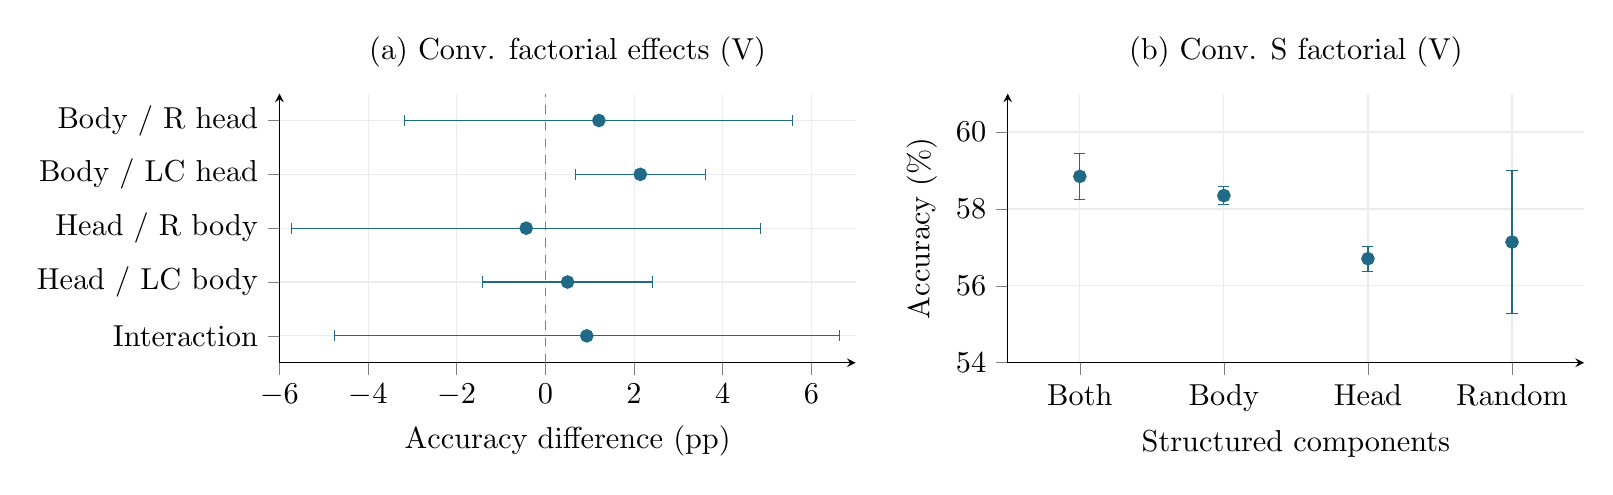
\begin{tikzpicture}
\begin{axis}[width=89mm,height=50mm,axis lines=left,tick align=outside,grid=major,grid style={gray!15},scaled ticks=false,tick label style={font=\fontsize{11}{13}\selectfont},label style={font=\fontsize{11}{13}\selectfont},title style={font=\fontsize{11}{13}\selectfont},legend style={font=\fontsize{11}{13}\selectfont,draw=none,fill=white,inner sep=1pt},title={(a) Conv. factorial effects (V)},xmin=-6,xmax=7,ymin=-.5,ymax=4.5,ytick={0,1,2,3,4},yticklabels={{Interaction},{Head / LC body},{Head / R body},{Body / LC head},{Body / R head}},xlabel={Accuracy difference (pp)}]
\draw[dashed,gray] (axis cs:0,-.5)--(axis cs:0,4.5);
\addplot+[color=methodblue,mark=*,mark size=2pt,line width=0.9pt,mark options={solid,fill=methodblue,draw=methodblue},only marks,error bars/.cd,x dir=both,x explicit] coordinates {(1.2066667,4) +- (4.3753515,0)};
\addplot+[color=methodblue,mark=*,mark size=2pt,line width=0.9pt,mark options={solid,fill=methodblue,draw=methodblue},only marks,error bars/.cd,x dir=both,x explicit] coordinates {(2.14,3) +- (1.466391,0)};
\addplot+[color=methodblue,mark=*,mark size=2pt,line width=0.9pt,mark options={solid,fill=methodblue,draw=methodblue},only marks,error bars/.cd,x dir=both,x explicit] coordinates {(-0.43333333,2) +- (5.2911933,0)};
\addplot+[color=methodblue,mark=*,mark size=2pt,line width=0.9pt,mark options={solid,fill=methodblue,draw=methodblue},only marks,error bars/.cd,x dir=both,x explicit] coordinates {(0.5,1) +- (1.9095497,0)};
\addplot+[color=methodblue,mark=*,mark size=2pt,line width=0.9pt,mark options={solid,fill=methodblue,draw=methodblue},only marks,error bars/.cd,x dir=both,x explicit] coordinates {(0.93333333,0) +- (5.6995577,0)};
\end{axis}
\begin{axis}[width=89mm,height=50mm,axis lines=left,tick align=outside,grid=major,grid style={gray!15},scaled ticks=false,tick label style={font=\fontsize{11}{13}\selectfont},label style={font=\fontsize{11}{13}\selectfont},title style={font=\fontsize{11}{13}\selectfont},legend style={font=\fontsize{11}{13}\selectfont,draw=none,fill=white,inner sep=1pt},at={(9.25cm,0)},anchor=south west,title={(b) Conv. S factorial (V)},xmin=-.5,xmax=3.5,ymin=54,ymax=61,xtick={0,1,2,3},xticklabels={Both,Body,Head,Random},xlabel={Structured components},ylabel={Accuracy (\%)}]
\addplot+[color=methodblue,mark=*,mark size=2pt,line width=0.9pt,mark options={solid,fill=methodblue,draw=methodblue},only marks,error bars/.cd,y dir=both,y explicit] coordinates {(0,58.846667) +- (0,0.60044428)};
\addplot+[color=methodblue,mark=*,mark size=2pt,line width=0.9pt,mark options={solid,fill=methodblue,draw=methodblue},only marks,error bars/.cd,y dir=both,y explicit] coordinates {(1,58.346667) +- (0,0.23860707)};
\addplot+[color=methodblue,mark=*,mark size=2pt,line width=0.9pt,mark options={solid,fill=methodblue,draw=methodblue},only marks,error bars/.cd,y dir=both,y explicit] coordinates {(2,56.706667) +- (0,0.32516662)};
\addplot+[color=methodblue,mark=*,mark size=2pt,line width=0.9pt,mark options={solid,fill=methodblue,draw=methodblue},only marks,error bars/.cd,y dir=both,y explicit] coordinates {(3,57.14) +- (0,1.8700802)};
\end{axis}
\end{tikzpicture}\end{document}
